\section*{¿Cómo funciona un sensor LiDAR?}

\subsection*{Tipo Topográfico:}
El sensorautoref\autoref{fig:TOP} posee un escáner que emite rayos infrarrojos que rebotan en las superficies con las que impactan, posteriormente los rayos que vuelven al sensor son registrados por un receptor y se realiza una medición en función del tiempo y la velocidad de la luz. El sensor LiDAR dispara miles de rayos por segundo los cuales generan la llamada nube de puntos, estos al combinarse con información posicional GPS/INS, genera un mapeo de puntos tridimensionales en tiempo real.\cite{NOAA_Lidar} 
\begin{figure}[h]
	\centering
	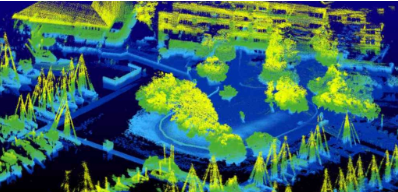
\includegraphics[width=0.3\linewidth]{img/TOP}
	\caption{Mapa topografico terrestre }
	\label{fig:TOP}
\end{figure}
\subsection*{Tipo Batimétrico:}
El sensor\autoref{fig:BAT} utiliza un escáner que emite luz verde, el cual es capaz de penetrar en el agua para hacer un mapeo completo de las profundidades costeras, lagos, ríos, etc. Con este tipo de escáner es posible detectar profundidades de hasta 10 metros.\cite{UAVLatam_Lidar}
\begin{figure}[h]
	\centering
	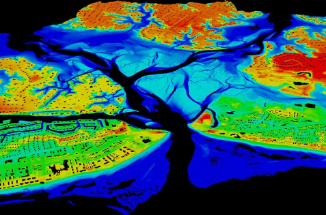
\includegraphics[width=0.3\linewidth]{img/BAT}
	\caption{Mapa de Lynnhavent,Virginia }
	\label{fig:BAT}
\end{figure}

Dicho escaneo puede tomar distintas formas:
\begin{itemize}
	\item Líneas: se producen líneas paralelas al momento de realizar el escaneado debido a que el sensor posee un espejo rotatorio que desvía el haz láser. 
	\item Zigzag: el espejo rotatorio produce líneas en forma de zigzag como patrón de escaneado debido a que el espejo es rotatorio en dos sentidos, ida y vuelta.  
	\item Fibra óptica: el haz láser es desviado desde un cable de fibra óptica, y el patrón de escaneado toma la forma de pequeñas circunferencias
	\item Elíptica: el patrón de escaneado toma forma elíptica, el cual se produce a través del desvío del haz láser por intermedio de dos espejos.
\end{itemize}

\subsection*{Componentes de un sensor LiDAR:}
\begin{itemize}
	\item Un escáner láser que emite pulsos rápidos de luz láser casi infrarroja
	\item Un sensor LiDAR utilizado para detectar y recoger los pulsos luminosos reflejados 
	\item Un procesador para calcular el tiempo y la distancia, así como para construir el conjunto de datos resultante, denominado nube de puntos LiDAR. 
\end{itemize}




